% vim: set spell spelllang=en tw=100 et sw=4 sts=4 :

\documentclass[a1paper]{tikzposter}

\usepackage{complexity}
\usepackage{wrapfig}
\usepackage{microtype}
\usepackage{tikz}
\usepackage{multicol}
\usepackage{colortbl}
\usepackage{booktabs}

\usepackage{lmodern}
\renewcommand*\familydefault{\sfdefault}
\usepackage[T1]{fontenc}

\title{Scheduling Match Races for Sailing}
\author{Craig Macdonald, Ciaran McCreesh, Alice Miller and Patrick Prosser}
\institute{University of Glasgow, Scotland ; c.mccreesh.1@research.gla.ac.uk}
\titlegraphic{
\includegraphics[keepaspectratio=true,scale=2.5]{UoG_keyline.pdf}}

\settitle{
    \begin{tikzpicture}
        \node (T) [inner sep=0pt] {\begin{minipage}{\linewidth}
                \color{titlefgcolor}
                {\bfseries \Huge \hspace{10mm}\@title \par}
                \vspace*{1em}
                {\large {\bfseries \hspace{10mm}\@author}\par}
                {\large {\hspace{10mm}\@institute}\par}
        \end{minipage}};

        \node at (T.east) [anchor=center, inner sep=0pt, xshift=-8cm] {\@titlegraphic};
    \end{tikzpicture}
}

% University of Glasgow standard colours
\definecolor{uofguniversityblue}{rgb}{0, 0.219608, 0.396078}

\definecolor{uofgheather}{rgb}{0.356863, 0.32549, 0.490196}
\definecolor{uofgaquamarine}{rgb}{0.603922, 0.72549, 0.678431}
\definecolor{uofgslate}{rgb}{0.309804, 0.34902, 0.380392}
\definecolor{uofgrose}{rgb}{0.823529, 0.470588, 0.709804}
\definecolor{uofgmocha}{rgb}{0.709804, 0.564706, 0.47451}

\definecolor{uofglawn}{rgb}{0.517647, 0.741176, 0}
\definecolor{uofgcobalt}{rgb}{0, 0.615686, 0.92549}
\definecolor{uofgturquoise}{rgb}{0, 0.709804, 0.819608}
\definecolor{uofgsunshine}{rgb}{1.0, 0.862745, 0.211765}
\definecolor{uofgpumpkin}{rgb}{1.0, 0.72549, 0.282353}
\definecolor{uofgthistle}{rgb}{0.584314, 0.070588, 0.447059}
\definecolor{uofgpillarbox}{rgb}{0.701961, 0.047059, 0}
\definecolor{uofglavendar}{rgb}{0.356863, 0.301961, 0.580392}

\definecolor{uofgsandstone}{rgb}{0.321569, 0.278431, 0.231373}
\definecolor{uofgforest}{rgb}{0, 0.317647, 0.2}
\definecolor{uofgburgundy}{rgb}{0.490196, 0.133333, 0.223529}
\definecolor{uofgrust}{rgb}{0.603922, 0.227451, 0.023529}

\definecolorstyle{UofG}{
}{
    % Background Colors
    \colorlet{backgroundcolor}{uofgsandstone!80!white}
    \colorlet{framecolor}{black}
    % Title Colors
    \colorlet{titlefgcolor}{white}
    \colorlet{titlebgcolor}{uofguniversityblue}
    % Block Colors
    \colorlet{blocktitlebgcolor}{white}
    \colorlet{blocktitlefgcolor}{uofguniversityblue}
    \colorlet{blockbodybgcolor}{white}
    \colorlet{blockbodyfgcolor}{black}
    % Innerblock Colors
    \colorlet{innerblocktitlebgcolor}{uofguniversityblue}
    \colorlet{innerblocktitlefgcolor}{black}
    \colorlet{innerblockbodybgcolor}{uofgsandstone!80!white}
    \colorlet{innerblockbodyfgcolor}{black}
    % Note colors
    \colorlet{notefgcolor}{black}
    \colorlet{notebgcolor}{uofgrust}
    \colorlet{noteframecolor}{red}
}

\usetheme{Autumn}
\usecolorstyle{UofG}

\tikzposterlatexaffectionproofoff

\useblockstyle[bodyverticalshift=-1cm, roundedcorners=1]{Default}

% Styles for drawings

\begin{document}
\maketitle

{
    \colorlet{blockbodybgcolor}{uofgcobalt}
    \colorlet{blocktitlebgcolor}{uofgcobalt}
    \block[bodyverticalshift=0cm, bodyinnersep=3mm]{}{
        \centering\begin{minipage}{0.9\textwidth}
            In sailing match races, \textbf{skippers race in pairs}. Each skipper races
            against each other skipper once, in a \textbf{round-robin} tournament. The
            order of matches in rounds is important: for example, a skipper who sails
            last in one round must not sail first in the following round. When there are fewer boats
            than skippers, \textbf{boats must be shared} and we would like to \textbf{minimise the
            number of boat changes}. We used \textbf{constraint programming} to develop
            \textbf{fairer schedules} for these competitions.
        \end{minipage}
    }
}

\begin{columns}
\column{0.5}

\block{Sailing Match Races}{
    \begin{center}
    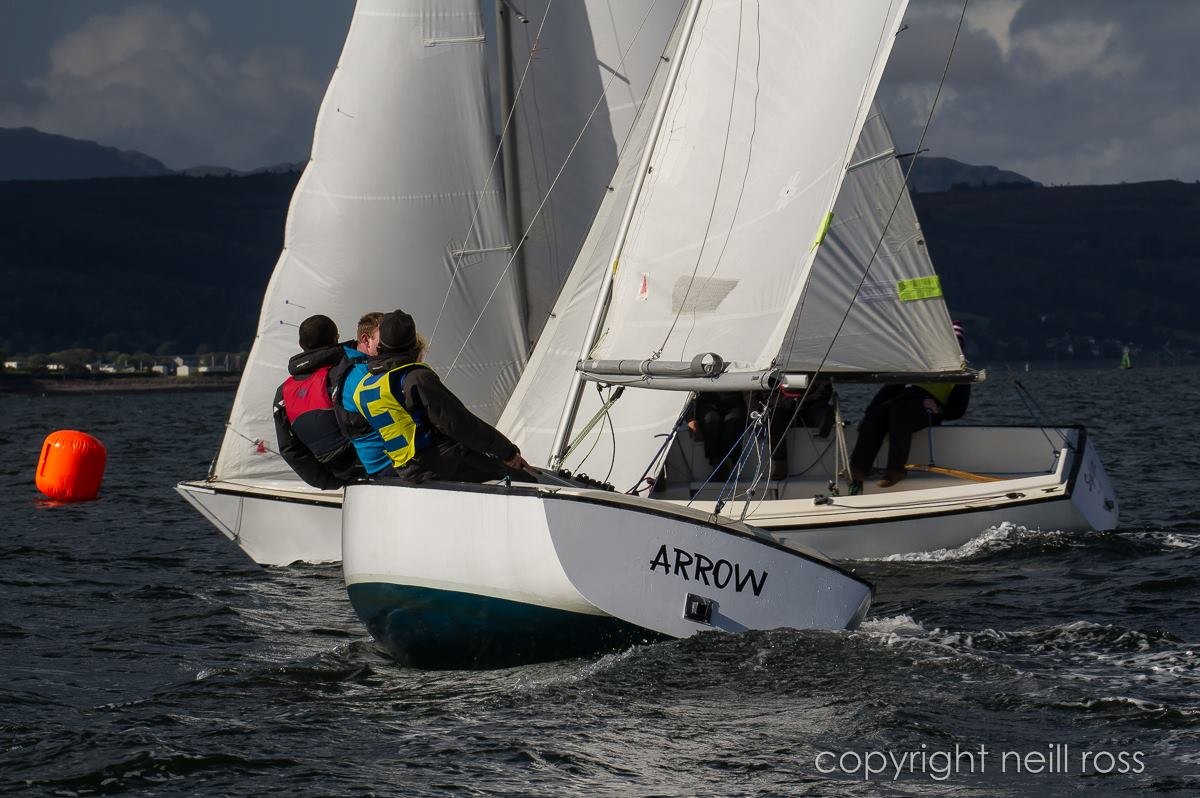
\includegraphics[keepaspectratio=true,width=0.93\linewidth]{photo.jpg}
    \end{center}

    \vspace*{0.6cm}

    In a match race, skippers races against each other in pairs. There are \textbf{several hundred
    events} per year, each involving up to ten of the 1,500 internationally registered skippers.
}

\block{Constraint Programming}{
    Constraint programming lets us describe a \textbf{model}, in terms of \textbf{variables}, a set
    of \textbf{constraints} between the variables, and an \textbf{objective}.
    We do \emph{not} need to provide an algorithm: we simply gave our model to the \textbf{Choco
    Solver} to solve.

    \bigskip

    For match racing, this let us focus on \textbf{understanding the problem} rather than designing
    an algorithm, and allowed us to develop a model \textbf{incrementally}, by adding in constraints
    in stages. Being able to use \textbf{expressive constraints} and \textbf{natural variable types}
    made our model easier to develop, easier to understand, and easier to verify.
}

\column{0.5}

\block{Round-Robin Schedules}{
    Sailing match race schedules are provided as \textbf{downloadable templates}, using numbers
    instead of skipper names. In each round, pairs of skippers race in a sequence of matches.

    \vspace*{0.5cm}

    \begin{center}
        \setlength{\tabcolsep}{6pt}
        \setlength{\aboverulesep}{0pt}
        \setlength{\belowrulesep}{0pt}
        \setlength{\extrarowheight}{.75ex}
        \begin{tabular}{c>{\columncolor{uofgcobalt}}c>{\columncolor{uofgpumpkin}}c>{\columncolor{uofglawn}}cc@{\hspace{2em}}c>{\columncolor{uofgcobalt}}c>{\columncolor{uofgpumpkin}}c>{\columncolor{uofglawn}}c}
            \toprule
            Round & \multicolumn{3}{c}{Matches} && Round & \multicolumn{3}{c}{Matches} \\[2pt] \midrule
            1 & (1,2) & (3,4) & (5,6) && 5 & (4,6) & (2,7) & (3,5) \\
            2 & (1,3) & (5,7) & (2,6) && 6 & (4,7) & (1,5) & (3,6) \\
            3 & (3,7) & (1,6) & (2,4) && 7 & (4,5) & (2,3) & (1,7) \\
            4 & (6,7) & (1,4) & (2,5) \\[4pt] \bottomrule
        \end{tabular}
    \end{center}

    \vspace*{0.5cm}

    The International Sailing Federation specifies what makes a legal match race schedule.  There
    are 13 criteria, and all existing schedules were \textbf{produced by hand}. This is a
    daunting task: \textbf{most are illegal}, many are missing, and some that are legal are
    \textbf{not as fair for competitors} as they could be.
}


\block{Channelling Between Perspectives}{
    When scheduling match races, some rules are temporal, some are described from a skipper's
    perspective, and some relate to rounds.

    \bigskip

    Constraint programming allows us to have \textbf{more than one model} of the problem, and we can
    express each constraint on whichever model is \textbf{most natural}. We then link the models
    using \textbf{channelling} constraints.

    \bigskip

    We used four models simultaneously for match racing. This was both \textbf{simpler}
    than a single model, and gave \textbf{better performance}.
}

\end{columns}

\block{Modelling Patterns in Sequences}{
    \begin{wrapfigure}[10]{r}{0.525\linewidth}
        \vspace{-2.5cm}\centering\begin{tikzpicture}

    \begin{scope}[every node/.style={minimum size=1.5em,inner sep=0.5}, scale=3]
        \node at (-0.5, 0) { ~ };
        \node (DFAS) [draw, circle, fill=white]                     at (0,  0)   { \small{S} };
        \node (DFAF) [draw, circle, fill=uofgcobalt]                at (2,  1.2) { \small{F} };
        \node (DFAM) [draw, circle, fill=uofgpumpkin]               at (2,  0)   { \small{M} };
        \node (DFAL) [draw, circle, fill=uofglawn]                  at (2, -1.2) { \small{L} };
        \node (DFAB) [draw, circle, fill=uofgthistle, text=white]   at (4,  0)   { \small{B} };
        \node (DFAE) [draw, circle, fill=uofgpillarbox, text=white] at (6,  0)   { \small{C} };

        \draw [->, >=latex, line width=2.5pt] (DFAS) to (DFAF);
        \draw [->, >=latex, line width=2.5pt] (DFAS) to (DFAM);
        \draw [->, >=latex, line width=2.5pt] (DFAS) to (DFAL);
        \draw [->, >=latex, line width=2.5pt] (DFAS) to [out=-20, in=-160] (DFAB);

        \draw [->, >=latex, line width=2.5pt] (DFAF) to [out=60, in=120, looseness=6] (DFAF);
        \draw [->, >=latex, line width=2.5pt] (DFAF) to [out=-125, in=125] (DFAL);
        \draw [->, >=latex, line width=2.5pt] (DFAF) to (DFAB);
        \draw [->, >=latex, line width=2.5pt] (DFAF) to [out=0, in=135] (DFAE);

        \draw [<->, >=latex, line width=2.5pt] (DFAF) to (DFAM);

        \draw [->, >=latex, line width=2.5pt] (DFAM) to [out=60, in=120, looseness=6] (DFAM);
        \draw [->, >=latex, line width=2.5pt] (DFAM) to [out=-25, in=-155] (DFAE);

        \draw [<->, >=latex, line width=2.5pt] (DFAM) to (DFAB);
        \draw [<->, >=latex, line width=2.5pt] (DFAM) to (DFAL);

        \draw [->, >=latex, line width=2.5pt] (DFAL) to [out=300, in=240, looseness=6] (DFAL);
        \draw [->, >=latex, line width=2.5pt] (DFAL) to [out=0, in=225] (DFAE);

        \draw [<-, >=latex, line width=2.5pt] (DFAL) to node [near start, xshift=0.7em] { $\star$ } (DFAB);

        \draw [->, >=latex, line width=2.5pt] (DFAB) to [out=30, in=-30, looseness=6] (DFAB);

        \draw [->, >=latex, line width=2.5pt] (DFAE) to [out=30, in=-30, looseness=6] (DFAE);
    \end{scope}

    \begin{scope}[xshift=14.5cm, yshift=-6cm, scale=0.5]
        \node [anchor=center, draw, rectangle split, rectangle split horizontal, rectangle split parts=7,
            rectangle split part fill={uofglawn,uofglawn,uofgpumpkin,uofgcobalt,uofgcobalt,uofglawn,uofgpillarbox}] at (0, 0) {
            \nodepart[text width=1em, align=center] {one}   \small{L}
            \nodepart[text width=1em, align=center] {two}   \small{L}
            \nodepart[text width=1em, align=center] {three} \small{M}
            \nodepart[text width=1em, align=center] {four}  \small{F}
            \nodepart[text width=1em, align=center] {five}  \small{F}
            \nodepart[text width=1em, align=center] {six}   \small{L}
            \nodepart[text width=1em, align=center, text=white] {seven} \small{C}
        };

        \node [anchor=center, draw, rectangle split, rectangle split horizontal, rectangle split parts=7,
            rectangle split part
        fill={uofgcobalt,uofglawn,uofglawn,uofglawn,uofgpumpkin,uofgthistle,uofgpumpkin}] at (0, -3) {
                \nodepart[text width=1em, align=center] {one}   \small{F}
                \nodepart[text width=1em, align=center] {two}   \small{L}
                \nodepart[text width=1em, align=center] {three} \small{L}
                \nodepart[text width=1em, align=center] {four}  \small{L}
                \nodepart[text width=1em, align=center] {five}  \small{M}
                \nodepart[text width=1em, align=center, text=white] {six}   \small{B}
                \nodepart[text width=1em, align=center] {seven} \small{M}
            };

        \node[anchor=center, draw, rectangle split, rectangle split horizontal, rectangle split parts=7,
            rectangle split part
        fill={uofgpumpkin,uofgthistle,uofglawn,uofgpumpkin,uofgcobalt,uofgcobalt,uofgcobalt}] at (0, -6) {
                \nodepart[text width=1em, align=center] {one}   \small{M}
                \nodepart[text width=1em, align=center, text=white] {two}   \small{B}
                \nodepart[text width=1em, align=center] {three} \small{L}
                \nodepart[text width=1em, align=center] {four}  \small{M}
                \nodepart[text width=1em, align=center] {five}  \small{F}
                \nodepart[text width=1em, align=center] {six}   \small{F}
                \nodepart[text width=1em, align=center] {seven} \small{F}
            };
    \end{scope}
    \end{tikzpicture}
    \end{wrapfigure}

    If a skipper is last out in one round, they must not go out first in the next round, to give
    them time to recover. Similar rules govern byes and boat changes. We model this using a sequence
    of states for each skipper, specifying whether that skipper is in first position, last,
    in the middle, in a bye, or has completed all their matches, for each round. The diagram shows
    which transitions are valid, with three examples---the automaton is used directly, as a
    $\mathit{regular}$ constraint on the sequence.

    \bigskip

    This kind of constraint is also used for scheduling suitable patterns of \textbf{day and night
    shifts} for staff rotas, and specifying \textbf{permitted sequences of jobs} on a production
    line.
}

{
    \colorlet{blockbodybgcolor}{uofgsandstone!80!white}
    \colorlet{blocktitlebgcolor}{uofgsandstone!80!white}
    \block[bodyverticalshift=-1.5cm]{}{\small
        Craig Macdonald, Ciaran McCreesh, Alice Miller, Patrick Prosser:
        \textbf{Constructing Sailing Match Race Schedules: Round-Robin Pairing Lists.} CP 2015:
        671-686. \\
        Photograph copyright Neill Ross, used with permission.
    }
}

\end{document}

